% \documentclass[10pt, oneside, english]{article}   	
\documentclass[10pt, oneside]{article}
\usepackage{geometry}                		
\geometry{a4paper}                   		
% \usepackage[english, es-noindentfirst]{babel}
% \selectlanguage{english}
\usepackage[utf8]{inputenc}               		
\usepackage{graphicx}			
\usepackage{amssymb}
\usepackage{authblk}
\usepackage{multicol}
\usepackage{rotating}
\usepackage{capt-of}
\usepackage{hyperref}	%autoref
\usepackage{amsmath}	%equation*
\usepackage{array}
\newenvironment{Figure}
	{\par\medskip\noindent\minipage{\linewidth}}
	{\endminipage\par\medskip}

\title{Word embeddings for predicting political affiliation based on Twitter data}

\author[]{Ibrahim Abdelaziz}
\author[]{Oliver Berg}
\author[]{Angjela Davitkova}
\author[]{Venkatesh Iyer}
\author[]{Shriram Selvakumar}
\author[]{Kumar Shridhar}
\author[]{Saurabh Varshneya}
\affil[1]{Technische Universität Kaiserslautern}

\date{\today}


\begin{document}
\maketitle
\begin{multicols}{2}


\section{Abstract}

Twitter as one of today's biggest social media platforms allows political figures to express their thinking easily and with a concise message. We propose a generic way of classifying political affiliation based on Twitter posts. This involves Word2Vec vector representations of the input data and utilizes pre-trained embeddings for the German language. With this we have shown to be capable of insightfully position German political figures in the political spectrum. 


\section{Introduction}

Social media platforms like \emph{Twitter} allows people of interest to communicate their personal opinion, and as such e.g. indicating political alignment, through a comprised message being only a few hundred character long. This yields broad potential to characterize personality traits such as political affiliation on.

Generally speaking, political motives were shown to be consistently predictable with an accuracy better than chance already \cite{Biessmann2017}.
This paper therefore proposes a \emph{deep learning} based classification model together with \emph{word embeddings} \cite{Pelevinala2016}. This allows a later analysis to find interesting constellations within the (German) political spectrum.
We leverage word embeddings to represent words in context. We thereby restrict ourselves to pre-trained models. Subsequently, a convolutional neural network (CNN) holistically classifies the Twitter profile by assigning each Twitter message a separate party label and combining these into a complete class score.


\section{Related Work}

Today, sentiment classification is mostly done using recurrent- or convolutional neural networks as described in \cite{Kim2014}. The presented approach uses a basic CNN trained on pre-trained word vector representations and does only little hyperparameter tuning to already achieve compelling results in question classification.

Additionally, \cite{Misra2016} introduces Recurrent Neural Networks (RNNs) for political bias analysis. Intuitively, RNNs operate more similar to how humans tend to process language: word by word, forming sentences. RNNs do train slower when compared to CNNs though, and CNNs generally produce more efficient representations of the data.

In connection to the given focus of working on Twitter data, \cite{Cohen2013} further introduces interesting questions concerning applicability of classification onto real data outside the training samples. It depicts the validation process as being prone to optimistic interpretations of the result when overlooking problems in latent attribute inference. This also suggests a critical view on this paper's final analysis results. 

In addition, \cite{SuggestedAdditionalResource2018} motivates context- and time dependencies within political data, which again makes analyzing an overall corpus of Twitter data a broadly connected issue.


\section{Methodology}

Formally, this paper proposes work on classifying Twitter data of political figures and picturing tendencies and dependencies within the data. As such, the following methodology is being applied. 

\subsection{Dataset} 

The dataset used in this approach was constructed of German politicians' Tweets posted on their Twitter accounts. 1000 German politicians' profiles with attributes "person name", "political party" and "twitter username" were retrieved from the website “https://www.wahl.de/”.
To reduce noise, only politicians belonging to the seven major political parties with respect to parliament activities, namely "CDU", "CSU", SPD", "FDP", "GRÜNE", "LINKE" and "AFD", are considered.

After the filtering stage this leaves a list of around 800 politicians, 125 of them are separated for the testing dataset. For each one up to 1000 of his/her most recent Tweets are gathered using Twitter API.

To prepare the Tweets for the training, and testing steps, each Tweet was preprocessed by first removing URLs, special characters, user names, and mentions. Then output empty Tweets are removed, and all characters are masked and put to lowercase.

Given the difference in the number of Tweets for each party, and in order to create a balanced training dataset, each party is restricted to a total of 12000 Tweets for training dataset, where each politician contributes approximately the same number of Tweets.

To represent the preprocessed Tweets text into numerical values that can be used to train, and test our model a pre-trained Word2Vec model is used \cite{DBLP:journals/corr/abs-1301-3781} - pre-trained on 200 million German Tweets \cite{cieliebak2017twitter} - which represent each word of the Tweet as a 200-dimensional vector.

\subsection{Classification}

The 200-dimensional word vectors are fed to a CNN model for classification.
The employed CNN architecture, shown in \autoref{fig:cnnArchitecture},  is based on \cite{Kim2014} which uses its model for sentiment analysis specifically. The resulting Tensorflow implementation is adapted by fine-tuning the hyper-parameters and adding dynamic learning rate for the given classification problem.

The first layers embeds words into low-dimensional vectors. Subsequent layers performs convolutions over the embedded word vectors using multiple filter sizes; sliding over 3, 4 and 5 words at a time. Max-pooling transforms the result of the constitutional layer into a long feature vector, dropout regularization with keep probability 0.5 is added and the result is classified using a final softmax-layer. We employed a dynamic learning rate between 0.005 to 0.0001 with exponential decay coefficient of 2.5 applied every epoch.

\begin{Figure}
	\centering
	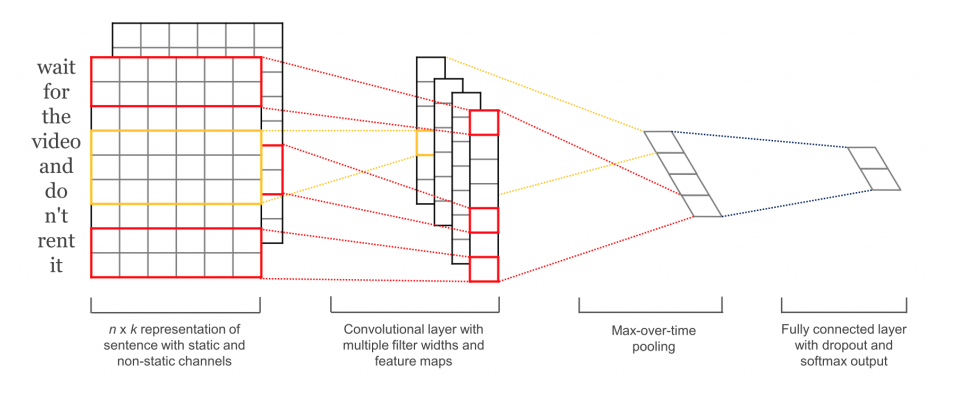
\includegraphics[width=\linewidth]{images/cnn_architecture1.png}
	\captionof{figure}{Model Architecture \cite{Wildml2015}}
	\label{fig:cnnArchitecture}
\end{Figure}

The overall classification process can be sub-divided into two elementary parts: First we \textbf{feed input data} to the neural network to then \textbf{classifying the (test-)data} for their respective classes.

In order to feed input data: For each party a raw text collection of all Tweets is considered. For each line - containing a single Tweet - a $<$PAD$>$ tokens is appended to achieve a fixed size length of size 35 which is the maximum word-length in a tweet for our dataset.  A vocabulary built on the complete corpus of existing words within the data maps each word to an integer between 0 and 109933 (number of existing words) for faster indexing.
Note that each Tweet is now represented as a vector of integers only. Using the pre-trained Word2Vec model, each Tweet can then be represented as a Matrix $M \in \mathbb{R}^{35 \times 200}$.

For classifying the user Tweets to the correct political party, we then feed the batches of twitter data along with their correct political party one-hot-encoded labels and train the above defined CNN. To optimize the network we use cross entropy loss defined as
\begin{equation*}
	H_{y'}(y) = - \sum_{i} y'_{i} \log (y_{i})
\end{equation*}
where $y$ is our predicted probability distribution, and $y'$ is the true distribution (the one-hot vector with the true-class party labels). 

\subsection{Analysis}\label{subsec:methodAnalysis}

To generally compare scoring accuracies across political parties 25 users per party are considered, where for each user a maximum of 200 Tweets (less if the total number of Tweets by the user is less than 200) are evaluated. Note here, that ultimately Tweets will be scored per person independently to then be combined to reach better generalization.

To numerically compare Tweets, each Tweet is characterized as a single sequence of words, where each word is represented as word vector from the word embedding space. The word sequence is then represented as the sentence vector (in $\mathbb{R}^200$) created by averaging all word vectors within that sentence.
Averaging word vectors is used instead of CNN computation results as the original messages should be compared rather than their formal characteristics / abstract features.
Note that Tweets containing $<$UNK$>$-tokens contain Twitter-specific functionality rather than natural language messages, and need to be removed from the overall sentence corpus.

For the visualization of results, sentence vectors were visualized using a Tensorflow built-in visualizer called the Embedding Projector that allows interactive visualization and analysis of high-dimensional data.
The high-dimensional vectors is reduced to 2 dimensional space using T-SNE and then the model is further visualized.

Additionally, to correctly visualize implicit dependencies between political parties, the ``political compass'' \cite{PoliticalCompass2017} representation is used for further visualizing the results. This incorporates a four way graph plot with attributes of ``Left-wing'' and ``Right-wing'' on the X-axis (Economic Scale), as well as ``Authoritarian'' and ``Libertarian'' on the Y-axis (Social Scale). Each party is positioned on the compass by a given X,Y coordinates - as is predefined in \cite{PoliticalCompass2017} - and associated figures are plotted on this given information plane.
The position of a given political figure is thereby influenced by the class labels of the person's Tweets as well as the relative positions of all parties on the Political Compass. Having obtained class labels for each Tweet of a person from the model classification (by choosing the class with the highest probability for the given Tweet), all of the person's Tweets belonging to the same parties are counted. Averaging all Tweet counters then results in the distribution over all classes. From this, the x-y-coordinates are calculated as a weighted sum of the distribution vector in relation to the x-y-coordinates of all the respective party positions on the political compass.


\section{Results}

Classification to a specific party based on a single tweet is a difficult task, even for humans. We, through our experiments comprehend the same as our results on individual tweets gave a low classification accuracy of 55 percent.
However, taking majority voting over a set of tweets for a given user led to a considerable increase in the classification accuracy as can be seen in \autoref{tbl:majorityVotingAccuracyScores}.

\begin{center}
	% \caption{Accuracy scores per party by majority voting}
	% \centering
	\begin{tabular}{|l|l|}
	\hline
	\textbf{political party} & \textbf{accuracy scores} \\ \hline
	AFD & 0.92 \\
	CSU & 0.84 \\
	FDP & 0.80 \\
	Die Grüne & 0.72 \\
	Die Linke & 0.88 \\
	SPD & 0.84 \\
	CDU & 0.72 \\
	\hline
	\end{tabular}
	\captionof{table}{Accuracy per party by majority voting}
	\label{tbl:majorityVotingAccuracyScores}
\end{center}

Concerning per-person visualization of political alignment as described in \autoref{subsec:methodAnalysis}, it was found that the visualizations over word-embeddings of tweets based on purely dimensionality reduction via T-SNE lacked a clear distinction between political party clusters. This was due to a given user's Re-Tweets to other parties to proclaim his presonal opinion on intra-party subject, resulting into a mixture of content across multiple parties.
This again motivated the utilization of formal political visualization techniques like the ``political compass''. Plotting the political representatives for each party onto the information plane yields an interesting constellation as can be seen in \autoref{fig:political_compass}.

\begin{Figure}
	\centering
	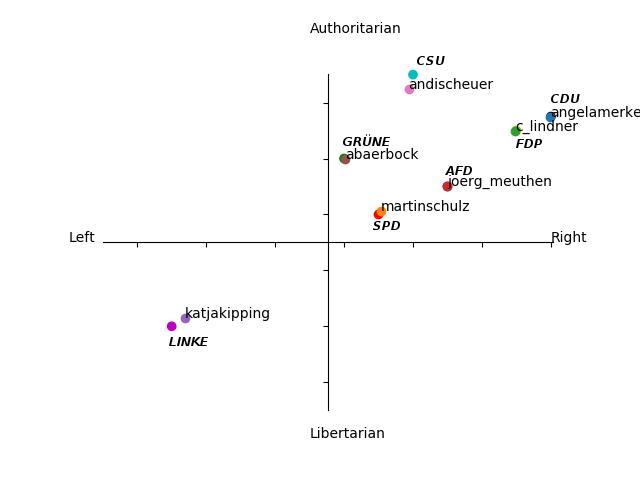
\includegraphics[width=\linewidth]{images/Political_Compass-final.png}
	\captionof{figure}{Plotting on Political Compass}
	\label{fig:political_compass}
\end{Figure}

Note here, that it was empirically verified that similar constellations of can be obtained with most other politicians from the depicted parties. Singular outliers were due to lack of holistic information disregarded.

By the example of \autoref{fig:political_compass} the following can be derived: Generally speaking, users appear close to their respective political party. Interestingly, the \emph{FDP}-class appears close to the \emph{CDU}-class, which concerning both parties' similar ideology was to be expected. In addition, very few users were strictly misclassified as not connecting to their own party's manifesto even though upon manual inspection appearing to very much share their party's strategies and intentions. This can be broken down to a huge number of $<$UNK$>$ tokens in the misclassified person's Tweets, due to e.g. non-German messages, frequent tag-like referencing or generally low numbers of Tweets. Outliers like these could be disregarded without distorting the overall picture.


\section{Conclusion}

As we have shown, a comparably simple convolutional neural network is able to nicely separate political figures concerning party affiliation.

Most politicians were found to appear close to the expected center of overall party orientation when pictured in the conceptually categorizing framework of the ``political compass''.

As the underlying word embeddings are taken from the German-language Wikipedia dump, we are currently restricted to German-language Tweets as well as to overall German-language features. This does suffice for general classification purposes, but poses the additional question of how the analysis would be affected if the embeddings were to be taken from \emph{intrinsically political} data samples. 
Also, our approach primarily focuses on CNNs and proves them to be efficient already. For future work, it would be intriguing to compare the capabilities of RNNs or other topologically different architectures. 

\end{multicols}

\newpage

\bibliography{lit}
\bibliographystyle{apalike}

\end{document} 
